\section{Materials and Methods}

\subsection{Literature review}

\subsubsection{Source of the literature}
The literature is fetched from PubMed (\url{https://pubmed.ncbi.nlm.nih.gov/})\cite{canese2013pubmed} and PubMed Central (PMC)\cite{roberts2001pubmed}. We searched in PubMed with the key word "acquired aplastic anemia" on \date{\today}. The title, year, abstract is downloaded using the "Save" function on PubMed searching page for further review.

\subsubsection{Word cloud plot}
The word cloud plot is done using \url{https://worditout.com/}. The input data are the selected abstracts of the reviewed articles.

\subsubsection{Selection of the literature}
The selection of the literature is done manually, according to the title and abstract of each article. Our selection standard is shown in the figure below.

\begin{figure}[H]
    \centering
    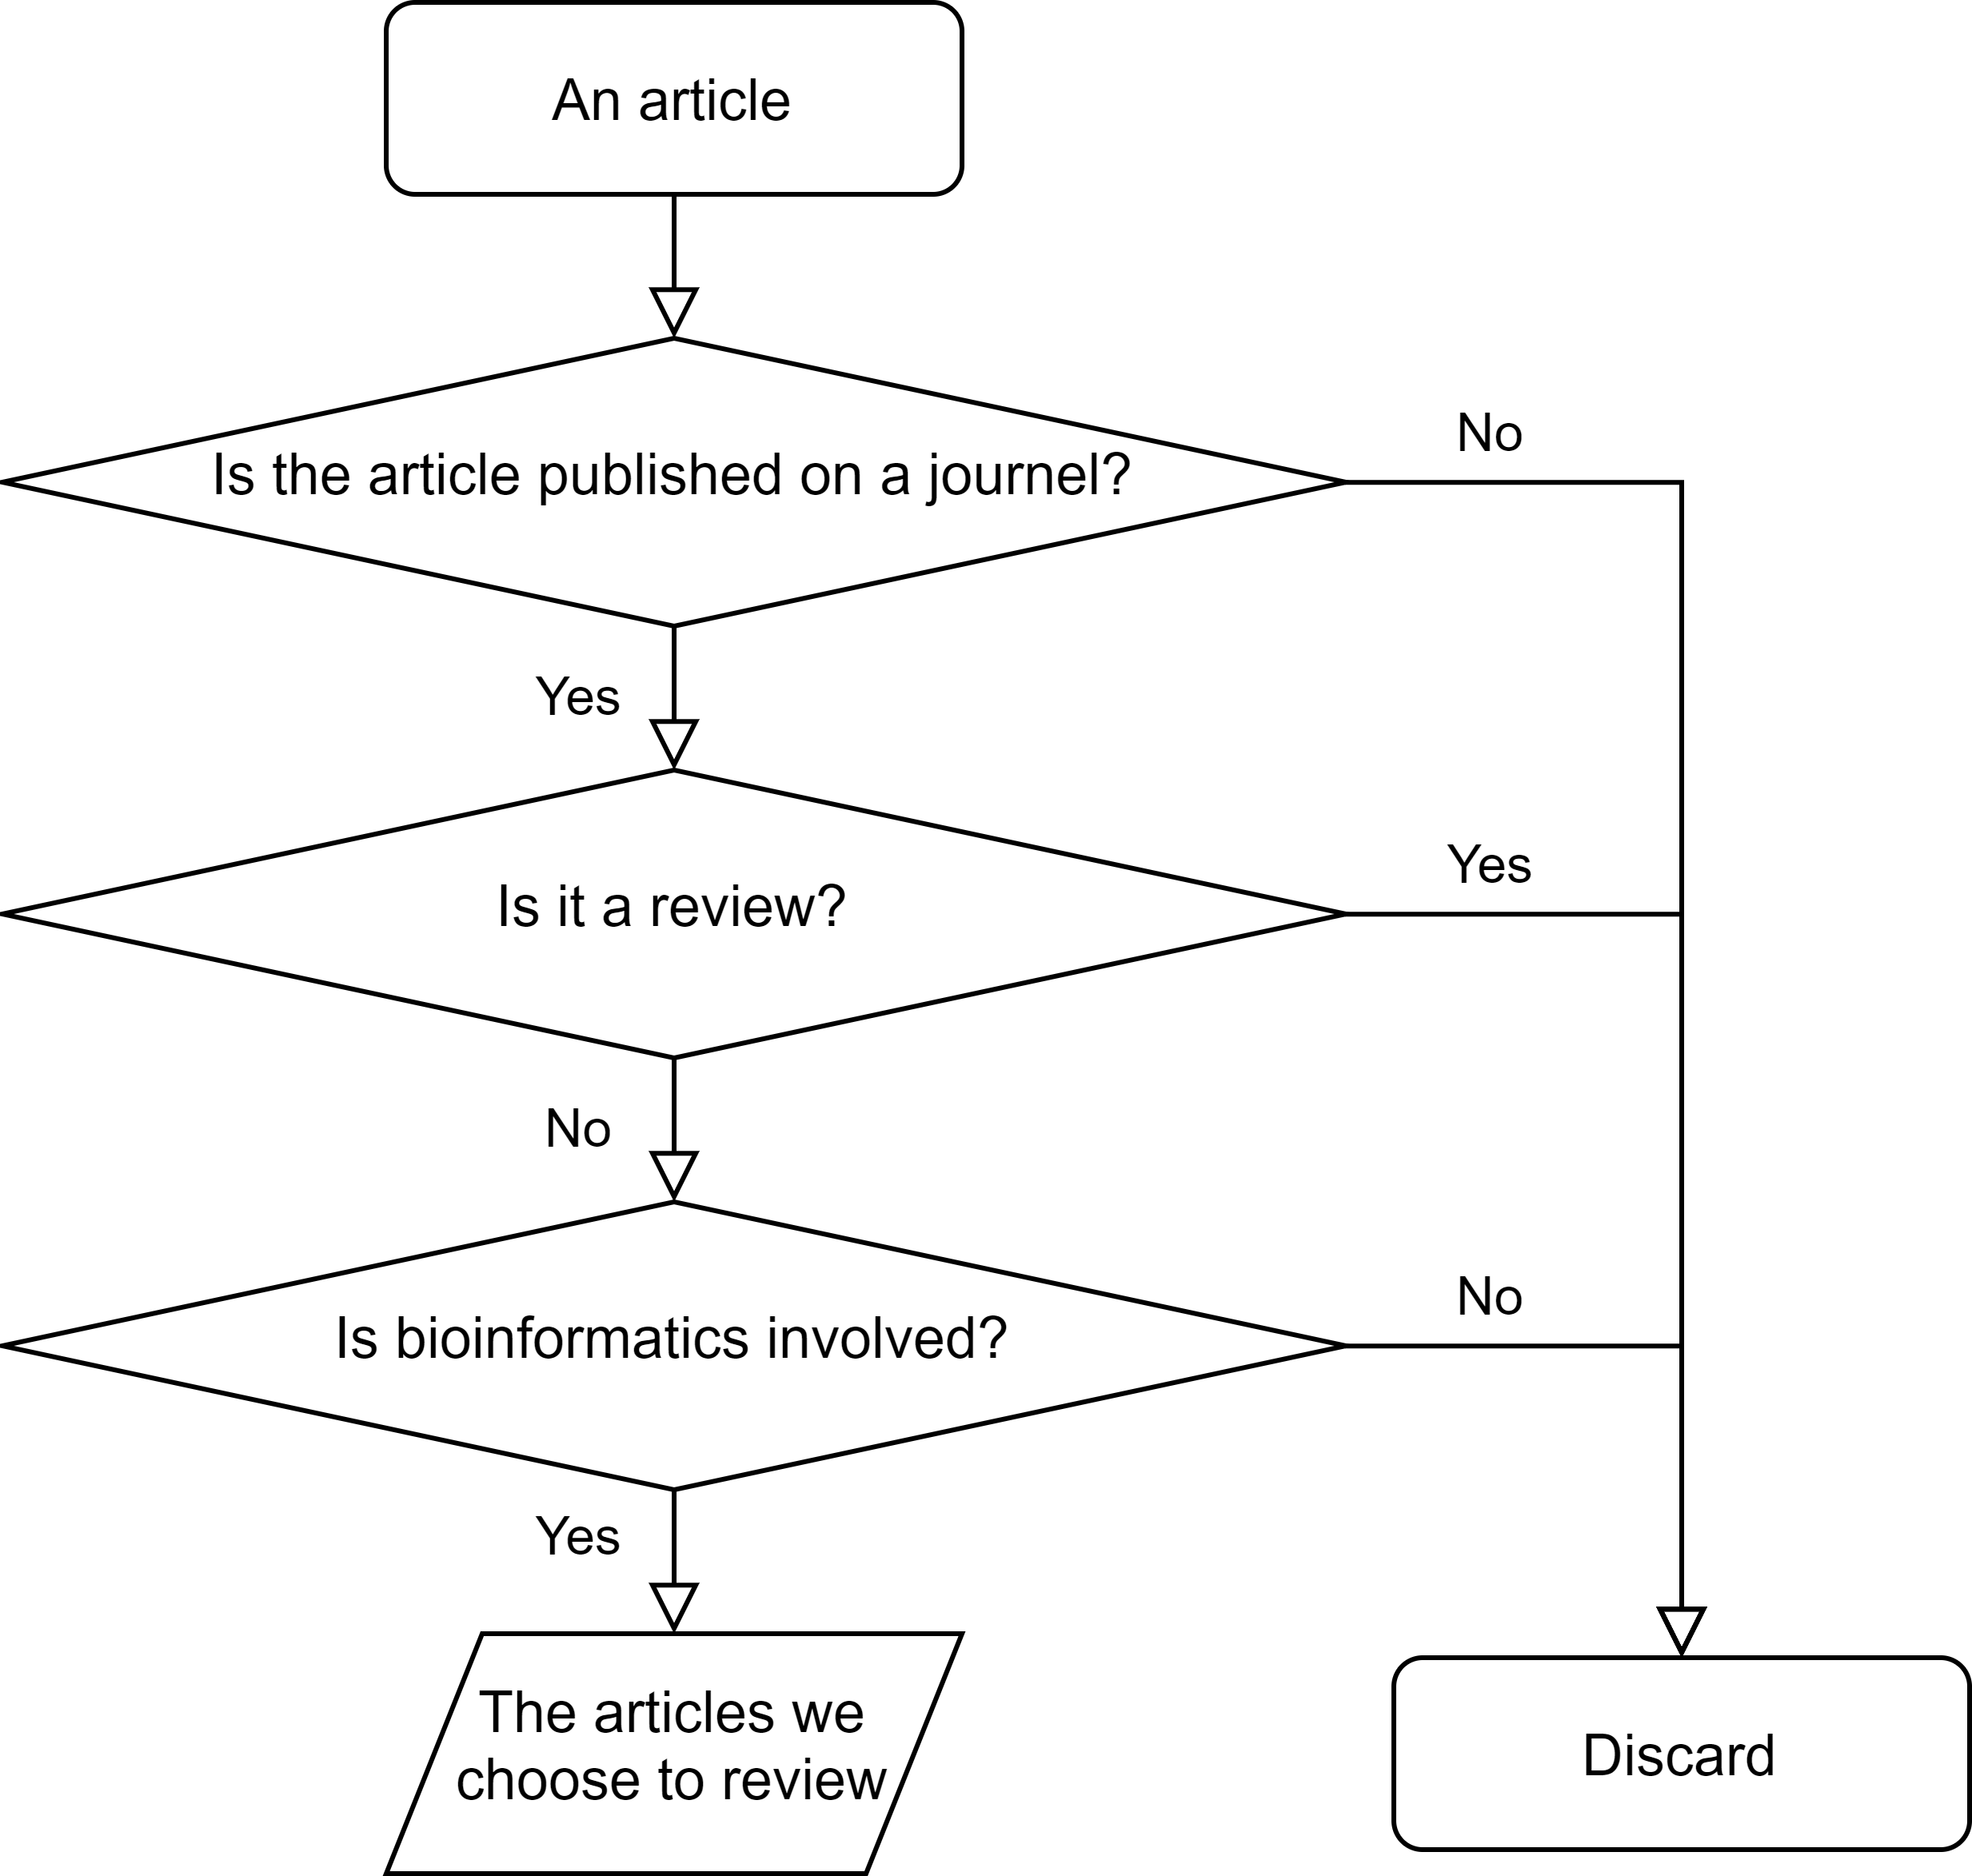
\includegraphics[width=0.4\textwidth]{image/Classification.png}
    \caption{Selection standard}
    \label{CS}
\end{figure}

\subsection{Transcriptomics analysis (Micro array data)}
\subsubsection{Data source}
The Micro array data used in Transcriptomics analysis is fetched from Gene Expression Omnibus (Gene Expression Omnibus), and the data set will be shown in the Results section.

\subsubsection{Tools and packages}
Transcriptomics analysis is done using R 4.0.5 with the following packages.

\begin{lstlisting}
library(Biobase)
library(GEOquery)
library(limma)
library(umap)
library("FactoMineR")
library("factoextra")
library(pheatmap)
\end{lstlisting}

Quality control of the data, selection of differently expressed genes, principal component analysis and heatmap plotting are done with the packages mentioned above. 

The standard of selection of differently expressed genes is $p\le 0.05$. Among all the differently expressed genes, the top 250 genes are used for principal component analysis and heatmap plotting.

Detailed configuration and code can be found in the Supplementary Material section.

\subsection{GO enrichment analysis}
\subsubsection{Data source}
The data used in GO enrichment analysis is fetched from Gene Expression Omnibus (Gene Expression Omnibus) , and the data set will be shown in the Results section. Annotation data of the GO enrichment comes from the R packages downloaded from Bioconductor\cite{gentleman2004bioconductor}.
\subsubsection{Tools and packages}
Transcriptomics analysis is done using R 4.0.5 with the following packages.

\begin{lstlisting}
library(org.Hs.eg.db)
library(clusterProfiler)
library(dplyr)
\end{lstlisting}

Results are shown in the form of dot plots, with p value and gene ratio labeled on the plot.

Detailed configuration and code can be found in the Supplementary Material section.
\subsection{Sequence analysis}
Sequence analysis is mostly done using online services like BLAST and ConservedDART\cite{geer2002cdart}. While the MSA is done using ClustalX 2.1\cite{larkin2007clustal}.

\subsection{Molecular docking}
The data used for docking is fetched from PDB and ZINC AC\cite{irwin2005zinc} (\url{https://zinc.docking.org/}). We did the molecular docking using the online service swissdock\cite{grosdidier2011swissdock}, with the parameters listed below.
\begin{lstlisting}
JOBNAME: 1PLF_Heparin
EMAIL: 1951510@tongji.edu.cn
PASSIVEFLEXIBILITYDISTANCE: 0.0
WANTEDCONFS: 5000
NBFACTSEVAL: 5000
NBSEEDS: 250
SDSTEPS: 100
ABNRSTEPS: 250
CLUSTERINGRADIUS: 2.0
MAXCLUSTERSIZE: 8
\end{lstlisting}

\subsection{Protein structure visualization}
Protein structure visualization is done using PDB online (Mol* Viewer\cite{sehnal2021mol}) and the visualization of docking results is done by UCSF Chimera\cite{pettersen2004ucsf}.

